\section{Métodos computacionales}

\subsection{Método DFTB}

\todo{Esto lo voy a pasar al capítulo de métodos, pero por ahora lo dejo acá...}


\subsection{Cálculos DFT}


\subsection{Algoritmo de ajuste}

\begin{figure}[h!]
    \centering
    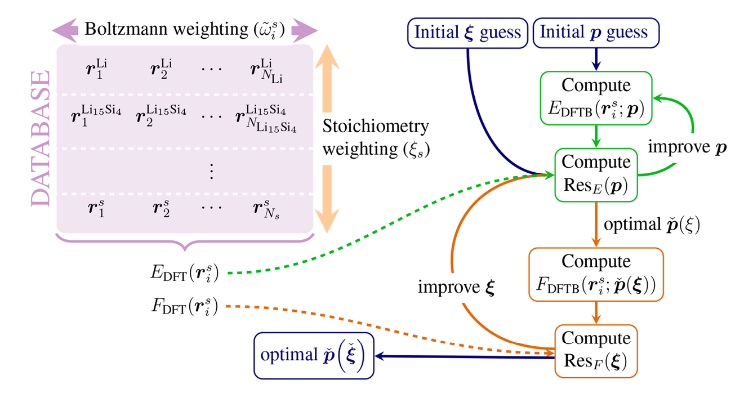
\includegraphics[width=\textwidth]{Silicio/modelo/metodos/diagrama.png}
    \caption{Diagrama de flujo del algoritmo de ajuste. Se realizan dos 
    procedimientos de optimización anidados: la minimización de Res$_E$ utilizando 
    el código TANGO \cite{tango} (resaltado en verde) y la minimización de Res$_F$
    utilizando un código llamado Milonga (resaltado en naranja). Cada mejora de 
    los pesos $\xi$ requiere una minimización completa de Res$_E$ para obtener 
    los parámetros óptimos DFTB asociados $\widecheck{p}(\xi)$.}
    \label{fig:diagrama}
\end{figure}
